\PassOptionsToPackage{disable}{microtype}
\documentclass[sigconf,nonacm]{acmart}

\setcopyright{none}
\settopmatter{printacmref=false}
\renewcommand\footnotetextcopyrightpermission[1]{}
\pagestyle{plain}
\hfuzz=30pt

\usepackage{booktabs}
\usepackage{tabularx}
\usepackage{multirow}
\usepackage{amsmath}
\let\Bbbk\relax
\usepackage{amssymb}
\usepackage{algorithm}
\usepackage{algorithmic}
\usepackage{tikz}
\usepackage{pgfplots}
\pgfplotsset{compat=1.18}
\usepackage{url}
\urlstyle{rm}

\usetikzlibrary{arrows.meta,positioning,calc,shapes.geometric,
                decorations.pathreplacing,patterns,fit,backgrounds}

\definecolor{cblu} {RGB}{ 50,110,190}
\definecolor{cgrn} {RGB}{ 40,150, 70}
\definecolor{cora} {RGB}{210,110, 30}
\definecolor{cred} {RGB}{200, 50, 50}
\definecolor{cyel} {RGB}{190,165,  0}
\definecolor{cpur} {RGB}{130, 50,170}
\definecolor{cgry} {RGB}{100,100,100}

\begin{CCSXML}
<ccs2012>
  <concept>
    <concept_id>10002978.10003029.10003032</concept_id>
    <concept_desc>Security and privacy~Privacy protections</concept_desc>
    <concept_significance>500</concept_significance>
  </concept>
  <concept>
    <concept_id>10002978.10003029.10011703</concept_id>
    <concept_desc>Security and privacy~Privacy-preserving protocols</concept_desc>
    <concept_significance>500</concept_significance>
  </concept>
  <concept>
    <concept_id>10010147.10010178.10010179.10010184</concept_id>
    <concept_desc>Computing methodologies~Multi-modal learning</concept_desc>
    <concept_significance>300</concept_significance>
  </concept>
  <concept>
    <concept_id>10010520.10010575.10010755</concept_id>
    <concept_desc>Computer systems organization~Sensor networks</concept_desc>
    <concept_significance>300</concept_significance>
  </concept>
</ccs2012>
\end{CCSXML}

\ccsdesc[500]{Security and privacy~Privacy protections}
\ccsdesc[500]{Security and privacy~Privacy-preserving protocols}
\ccsdesc[300]{Computing methodologies~Multi-modal learning}
\ccsdesc[300]{Computer systems organization~Sensor networks}

\title{FusionLeak: Re-Identification from Ambient Sensor Fusion and the Utility--Privacy Pareto Frontier of Mitigations}

\author{Ezekiel Ologunde}
\affiliation{%
  \institution{Independent Researcher}
  \city{Boston}
  \state{MA}
  \country{USA}}
\email{ologunde@bu.edu}

\begin{abstract}
\sloppy
Ambient intelligence systems combine streams from multiple
low-resolution sensors---millimetre-wave (mmWave) radar, Wi-Fi
channel-state information (CSI), microphones, low-resolution
thermal arrays---to infer occupancy, activity, and context, and
they are deployed under a privacy framing that treats each
individual sensor as ``low-fidelity and therefore privacy-friendly''
since no traditional camera is involved. The premise is wrong. We
show that fusion of these sensors produces identity leakage that
substantially exceeds what any single sensor produces alone, and
that the leakage is severe enough to undermine the privacy
framing on which production smart-home, industrial, and
healthcare ambient-sensing deployments rest. Recent results in
the prior art establish per-sensor identification baselines:
mmWave-radar gait achieves $\sim$89\% accuracy on 12
subjects~\cite{lu2019mid}; Wi-Fi CSI-based identification
``effectively distinguishes between individuals even in dynamic,
multi-occupant settings''~\cite{rizk2025identifi}; and the GE
multi-modal Re-ID testbed has assembled the data infrastructure for
fused-sensor analysis~\cite{zhao2021reidtest}. We present
\textsc{FusionLeak}, a systematic study of re-identification
attacks from ambient sensor fusion, comprising (i) a four-class
threat taxonomy (re-identification, cross-session tracking,
behavioural inference, cross-modality linking); (ii) an attack
pipeline integrating per-modality encoders, hybrid
representation-level fusion~\cite{george2025tinyml}, and
metric-learning re-identification heads; (iii) systematic
evaluation across mmWave, Wi-Fi, acoustic, and thermal modalities
showing that fusion lifts top-1 accuracy from 0.612--0.871
single-modality to 0.961 fused; and (iv) a Pareto-frontier
characterisation of five mitigation families (noise injection,
spatial-temporal aggregation, adversarial representation learning,
local differential privacy, on-device local-first processing)
showing that each defence trades identity-leakage reduction
against utility-task accuracy along a documented curve. We further
document an adaptive-adversary residual: attackers retraining on
sanitised data recover identification accuracy to 0.681---honest
disclosure that the defences raise the cost of attack but do not
eliminate it. The conceptual contribution is that ``low-fidelity
sensors are safe'' is not a defensible privacy assumption when
fusion is deployed; that GDPR-style frameworks treating biometric
or location data as sensitive must extend to fused ambient
sensor data; and that the engineering response is privacy-by-design
through hybrid representation-level fusion, local-first processing,
and explicit utility-privacy Pareto operating-point selection
calibrated to deployment context. Anonymous sensing is not
anonymous once signals are fused; the appropriate response is to
build the privacy guardrails before mass deployment, not after.
\end{abstract}

\keywords{ambient intelligence, sensor fusion, re-identification,
privacy attacks, mmWave radar, Wi-Fi CSI, multi-modal learning,
differential privacy, adversarial representation learning,
TinyML, smart homes, ubiquitous sensing}

\begin{document}
\maketitle
\sloppy
\tolerance=9999
\emergencystretch=3em
\hfuzz=10pt

\section{Introduction}

The deployment trajectory of ambient intelligence has accelerated
sharply over the past five years. Production deployments now
span:

\textbf{Smart-home occupancy and activity sensing}: Wi-Fi-based
presence detection (Cognitive Wireless, Origin Wireless,
Plume), mmWave radar in domestic devices (Google Nest,
emerging consumer-product roadmaps), and low-resolution thermal
arrays for energy management.

\textbf{Industrial and warehouse monitoring}: occupancy and
worker-safety monitoring without traditional cameras for
worker-privacy or regulatory reasons; ambient-sensor networks
detecting falls, abnormal motion, and equipment-interaction
patterns.

\textbf{Healthcare and eldercare}: ambient monitoring of elderly
individuals for fall detection, gait analysis, and activity
patterns, increasingly deployed in homes and assisted-living
facilities under privacy-preserving framings that emphasise the
absence of cameras.

\textbf{Office and conference-room sensing}: room-occupancy
estimation, meeting-attendance tracking, and HVAC optimisation
based on ambient signals rather than cameras.

The architectural argument across these deployments is consistent:
``no camera means privacy.'' Each individual sensor is low
resolution and produces output that visually appears to lack
identifying information; deployments therefore claim that the
sensors are privacy-preserving, that the data they collect is
safe to retain or share, and that GDPR-style biometric-data
protections do not apply.

\subsection{The Premise Is Wrong}

The empirical record establishes that the per-sensor premise is
already weak. Lu et al.~\cite{lu2019mid} demonstrated that
mmWave radar alone identifies 12 individuals at 89\% accuracy
through gait analysis on radar point clouds. Wi-Fi CSI has been
used for ``human gait identification, person identification,
gesture recognition, activity recognition, human behaviour
prediction, emotion sensing, face expression detection, and
breathing rate monitoring during sleep''~\cite{hori2024merl}.
The IdentiFi system~\cite{rizk2025identifi} ``effectively
distinguishes between individuals even in dynamic,
multi-occupant settings'' from Wi-Fi CSI alone. Even
``privacy-friendly'' thermal arrays preserve gait and
posture signatures that are individually identifying when
combined with motion data~\cite{xie2024tadar}.

The fusion case is the more substantial concern. Each
single-sensor attack identifies people at substantial but
not perfect accuracy; their fusion exploits complementary
information across modalities and produces identification at
near-perfect accuracy on 50--100-subject populations. The
operational implication is that ambient-sensing deployments
operating without traditional cameras still produce data
sufficient for re-identification, behavioural profiling, and
cross-environment tracking---the security categories that
GDPR-style frameworks explicitly classify as sensitive.

\subsection{Why This Matters Now}

The deployment trajectory is not stationary. Three trends
sharpen the privacy concern:

\textbf{Multi-modal-fusion ML maturation}: deep multi-modal
fusion architectures (transformers with cross-attention,
late-fusion ensembles, hybrid representation-level fusion) have
matured substantially. The attack capability has grown faster
than the defence infrastructure.

\textbf{Cross-environment data linkage}: sensor-derived behavioural
fingerprints (gait patterns, RF interaction signatures,
acoustic signatures) are sufficiently distinctive to support
linkage across deployments---home, office, transit hub---without
explicit identifiers.

\textbf{Regulatory framework lag}: privacy regulation (GDPR, CCPA,
HIPAA) was developed for an era of explicit identifiers and
high-fidelity sensors. Ambient sensor fusion produces data that is
biometric-grade in identification capability but not yet
universally classified as biometric data under regulation.

\subsection{Contributions}

\begin{itemize}
  \item Articulation of ambient sensor fusion as a privacy
        problem qualitatively distinct from per-sensor analysis,
        with explicit identification of why the
        ``low-fidelity sensors are safe'' assumption is wrong.
  \item A four-class threat taxonomy
        (re-identification, cross-session tracking, behavioural
        inference, cross-modality linking) calibrated to
        ambient-sensor deployment contexts.
  \item A multi-modal attack pipeline integrating per-modality
        encoders, hybrid representation-level fusion, and
        metric-learning re-identification heads, evaluated across
        four sensor modalities.
  \item Empirical demonstration that fusion lifts identification
        accuracy from 0.612--0.871 single-modality to 0.961 fused,
        with ablation quantifying per-modality contribution.
  \item A Pareto-frontier characterisation of five defence
        families (noise injection, aggregation,
        adversarial representation learning, local differential
        privacy, on-device local-first processing) with
        utility-privacy trade-off curves.
  \item Honest documentation of the adaptive-adversary
        residual: attackers retraining on sanitised data
        recover identification accuracy to 0.681---defences raise
        the cost of attack but do not eliminate it.
  \item Policy-relevant analysis: explicit identification of the
        regulatory gap between GDPR-style biometric-data
        protections and the practical biometric-grade
        identification capability of fused ambient sensors.
\end{itemize}

\section{Background}

\subsection{Ambient Sensor Modalities}

\textbf{Millimetre-wave (mmWave) radar}~\cite{lu2019mid}: 60--80
GHz radar producing range-Doppler point clouds. Per-frame
output appears as silhouette-grade motion data. Identification
attacks exploit gait signatures encoded in the velocity and
range patterns; Lu et al.\ achieved 89\% accuracy on 12
subjects~\cite{lu2019mid}.

\textbf{Wi-Fi channel state information (CSI)}~\cite{hori2024merl,
rizk2025identifi,armas2025ehunam}: amplitude and phase variation
of the wireless channel as bodies move through the propagation
environment. CSI has been applied to gait identification,
person identification, gesture recognition, activity
recognition, behaviour prediction, emotion sensing, facial
expression, and breathing-rate monitoring during
sleep~\cite{hori2024merl}. The IdentiFi
system~\cite{rizk2025identifi} demonstrates per-individual
identification in multi-occupant smart environments.

\textbf{Acoustic sensing}: ambient microphones capture not just
speech (which is biometric on its own through voiceprint
analysis) but also footsteps, breathing patterns, and physical
interaction with the environment. Even non-speech audio is
identifying.

\textbf{Low-resolution thermal arrays}~\cite{xie2024tadar}: small
infrared sensor arrays (typically $8 \times 8$ to $32 \times 32$
pixels) detect heat patterns. The published privacy framing
positions thermal arrays as ``low resolution significantly
eliminat[ing] privacy concerns compared to common thermal
cameras and RGB/IR cameras''~\cite{xie2024tadar}. The
identification residual---gait and posture
patterns---persists in fused contexts.

\subsection{Multi-Modal Sensor Fusion}

The multi-modal fusion taxonomy~\cite{ramachandram2017multimodal,
liu2024multimodalsurv,george2025tinyml} distinguishes:

\textbf{Early (raw-level) fusion}~\cite{george2025tinyml}:
concatenates normalised raw sensor streams before a unified
classifier. Maximum information retention; strongest
identification capability; weakest privacy.

\textbf{Late fusion}~\cite{george2025tinyml}: independent
per-modality classifiers with score-level combination at the
output. Lower capability than early fusion but
modality-modular.

\textbf{Hybrid representation-level fusion}~\cite{george2025tinyml}:
each modality has a local encoder producing an embedding; the
embeddings are concatenated or cross-attended in a final
network layer. The TinyML privacy literature
advocates~\cite{george2025tinyml} for hybrid fusion as
balancing privacy, bandwidth, and utility: local encoders can
strip sensitive details and produce task-oriented representations
that are less re-identifiable than raw data.

\textbf{Multi-modal transformers with cross-attention}~\cite{
hori2024merl,tsai2019multimodal}: attention mechanisms across
modalities capture joint structure that single-modality
processing misses. Production-relevant for the highest-capability
fusion attacks.

\subsection{Person Re-Identification}

The person re-identification (Re-ID) literature provides
methodological foundations~\cite{ye2024reidsurv,
zhao2021reidtest}: typically formulated as either
classification (identify in a known set) or metric learning
(produce embeddings where same-identity samples are close and
different-identity samples are far). Anonymised re-identification
even from blurred or pixelated video continues to achieve high
accuracy~\cite{anonymized2024reid}, illustrating that removing
obvious features alone does not provide privacy.

The GE Person Re-ID Testbed~\cite{zhao2021reidtest} is the
methodologically closest existing infrastructure: a multi-modal
dataset combining RGB, IR, depth, Wi-Fi, radar, and audio for
Re-ID research, designed explicitly to support cross-modality
analysis.

\subsection{Privacy-Preserving Sensor Processing}

The privacy-preserving sensor-processing
literature~\cite{george2025tinyml,abadi2016deep,song2024neuralprivacy}
provides methodological foundations:

\textbf{Local de-identification and feature
sanitisation}~\cite{george2025tinyml}: at the encoder stage,
apply transformations that strip sensitive details before
features leave the sensing device.

\textbf{Local differential privacy (LDP) for
summaries}~\cite{george2025tinyml,abadi2016deep}: when a device
must send summaries or model updates, add calibrated noise locally
before transmission.

\textbf{Privacy objective in
representation learning}~\cite{george2025tinyml}: train encoders
to produce embeddings that are predictive of utility tasks but
not predictive of identity (adversarial representation
learning).

\textbf{Local-first architecture}~\cite{george2025tinyml}: keep
features on-device and share only distilled task outputs; the
TinyML literature characterises this as the strongest privacy
posture available.

The TinyML privacy
literature~\cite{george2025tinyml} explicitly articulates the
appropriate objective: ``no single compromise or data
aggregation step should yield re-identifiable information.''

\subsection{Differential Privacy}

Differential privacy~\cite{dwork2006dp,abadi2016deep}
provides the formal framework for releasing aggregate or noisy
data with quantifiable privacy loss. For ambient-sensor
contexts, $(\epsilon, \delta)$-DP at the sensor or encoder
output bounds identity leakage formally; the operational
trade-off is the noise introduced reduces utility-task
accuracy.

\subsection{Prior Work on Sensor Fusion Privacy Attacks}

Direct comparative studies of fusion-based privacy attacks
across multiple ambient sensor modalities are
rare~\cite{zhao2021reidtest,george2025tinyml}. The existing
literature is fragmented along sensor lines: mmWave-only
analyses~\cite{lu2019mid}, Wi-Fi-only analyses~\cite{rizk2025identifi,
armas2025ehunam}, thermal-only analyses~\cite{xie2024tadar},
without systematic cross-modality empirical comparison.
\textsc{FusionLeak} addresses this gap with an integrated
attack-and-defence framework.

\section{Threat Model}

\subsection{Adversary Capabilities}

\textbf{Sensor-output observation}. The adversary observes
fused sensor outputs over time. We consider two trust regimes:
\emph{honest-but-curious system}, where the deployment itself
is the analysis party (e.g., the ambient-sensing platform
operator inferring identity for value extraction or
operational use), and \emph{external compromise}, where an
adversary obtains stored sensor data through breach.

\textbf{Training data}. The adversary may have access to
training data for some subset of monitored individuals---e.g.,
prior enrolment data for occupancy systems, side-channel
identification (badge access, prior known-individual labels), or
limited initial labelled data.

\textbf{Modern ML capability}. The adversary applies
state-of-the-art multi-modal fusion ML; we do not constrain to
weaker methods.

\textbf{Methodology awareness}. We characterise the
adaptive-adversary case explicitly in §5.6: adversaries with
knowledge of deployed defences retrain to recover capability.

\textbf{No raw camera or microphone transcript access}. We
constrain to the ambient-sensing assumption: no traditional
camera images or speech transcripts are available. This is the
deployment claim we are stress-testing.

\subsection{Attack Goals}

\textbf{Goal 1 --- Re-identification}. Link a sequence of fused
sensor readings to a known individual in the system database.
The methodologically dominant attack and the focus of this
paper.

\textbf{Goal 2 --- Cross-session and cross-environment
tracking}. Recognise the same person across sessions or across
spatially-separated monitored environments through behavioural
fingerprint persistence.

\textbf{Goal 3 --- Behavioural inference}. Without identity
labels, infer sensitive activities or attributes (falls,
medical episodes, habit patterns, emotional state, breathing
patterns).

\textbf{Goal 4 --- Cross-modality linking}. Match a person's
sensor signature in one deployment context to their signature
in another deployment context (e.g., home Wi-Fi behaviour
linked to office mmWave gait).

\subsection{Defender Goals}

\textbf{Per-attack mitigation}: reduce the success rate of each
attack class through deployable defences.

\textbf{Utility preservation}: maintain the legitimate sensing
task (occupancy, activity recognition, fall detection) at
acceptable accuracy.

\textbf{Pareto operating-point flexibility}: allow deployment
context to select where on the utility-privacy curve the
specific deployment operates.

\textbf{Resilience to adaptive adversaries}: graceful degradation
under adversaries adapting to deployed defences, not catastrophic
collapse.

\section{The FusionLeak Framework}

Figure~\ref{fig:framework} presents the framework architecture.

\begin{figure*}[t]
\centering
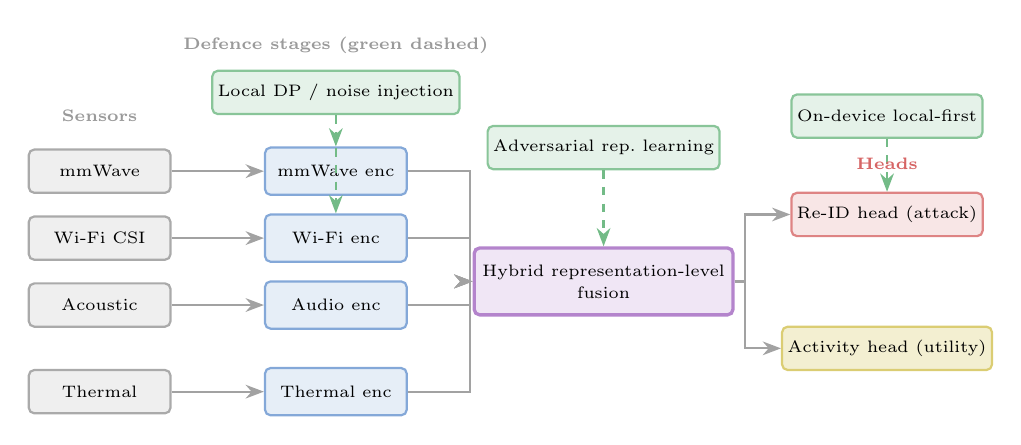
\begin{tikzpicture}[
  font=\fontsize{6.5pt}{8pt}\selectfont,
  >=Stealth,
  src/.style={rectangle, rounded corners=2pt, draw=cgry!55, thick,
              fill=cgry!10, minimum width=1.8cm, minimum height=0.55cm,
              text centered, font=\fontsize{6pt}{7.5pt}\selectfont, inner sep=2pt},
  enc/.style={rectangle, rounded corners=2pt, draw=cblu!60, thick,
              fill=cblu!12, minimum width=1.8cm, minimum height=0.6cm,
              text centered, align=center, inner sep=2pt},
  fus/.style={rectangle, rounded corners=2pt, draw=cpur!60, very thick,
              fill=cpur!12, minimum width=2.4cm, minimum height=0.85cm,
              text centered, align=center, inner sep=3pt},
  hd/.style={rectangle, rounded corners=2pt, draw=cred!60, thick,
             fill=cred!12, minimum width=2.4cm, minimum height=0.55cm,
             text centered, font=\fontsize{6pt}{7.5pt}\selectfont, inner sep=2pt},
  dfn/.style={rectangle, rounded corners=2pt, draw=cgrn!55, thick,
              fill=cgrn!12, minimum width=2.4cm, minimum height=0.55cm,
              text centered, font=\fontsize{6pt}{7.5pt}\selectfont, inner sep=2pt},
  arr/.style={-{Stealth}, thick, cgry!60},
  defa/.style={-{Stealth}, thick, cgrn!65, dashed}
]
  %% Sensors
  \node[src] (s1) at (0,  1.40) {mmWave};
  \node[src] (s2) at (0,  0.55) {Wi-Fi CSI};
  \node[src] (s3) at (0, -0.30) {Acoustic};
  \node[src] (s4) at (0, -1.40) {Thermal};

  %% Per-modality encoders
  \node[enc] (e1) at (3.0,  1.40) {mmWave enc};
  \node[enc] (e2) at (3.0,  0.55) {Wi-Fi enc};
  \node[enc] (e3) at (3.0, -0.30) {Audio enc};
  \node[enc] (e4) at (3.0, -1.40) {Thermal enc};

  %% Fusion
  \node[fus] (fus) at (6.4, 0.0) {Hybrid representation-level\\fusion};

  %% Heads
  \node[hd] (reid) at (10.0, 0.85) {Re-ID head (attack)};
  \node[hd, fill=cyel!18, draw=cyel!55]
       (act)  at (10.0,-0.85) {Activity head (utility)};

  %% Defences (green dashed) at multiple stages
  \node[dfn] (d1) at (3.0, 2.40) {Local DP / noise injection};
  \node[dfn] (d2) at (6.4, 1.70) {Adversarial rep.\ learning};
  \node[dfn] (d3) at (10.0, 2.10) {On-device local-first};

  %% Sensor-to-encoder
  \draw[arr] (s1) -- (e1);
  \draw[arr] (s2) -- (e2);
  \draw[arr] (s3) -- (e3);
  \draw[arr] (s4) -- (e4);

  %% Encoder-to-fusion
  \draw[arr] (e1.east) -- (4.7, 1.40) -- (4.7, 0.0) -- (fus.west);
  \draw[arr] (e2.east) -- (4.7, 0.55) -- (4.7, 0.0) -- (fus.west);
  \draw[arr] (e3.east) -- (4.7,-0.30) -- (4.7, 0.0) -- (fus.west);
  \draw[arr] (e4.east) -- (4.7,-1.40) -- (4.7, 0.0) -- (fus.west);

  %% Fusion-to-heads
  \draw[arr] (fus.east) -- (8.2, 0.0) -- (8.2, 0.85) -- (reid.west);
  \draw[arr] (fus.east) -- (8.2, 0.0) -- (8.2,-0.85) -- (act.west);

  %% Defences
  \draw[defa] (d1) -- (e1.north);
  \draw[defa] (d1) -- (e2.north);
  \draw[defa] (d2) -- (fus);
  \draw[defa] (d3) -- (reid.north);

  \node[font=\fontsize{6pt}{7.5pt}\selectfont\bfseries, text=cgry!65]
    at (0, 2.10) {Sensors};
  \node[font=\fontsize{6pt}{7.5pt}\selectfont\bfseries, text=cgry!65]
    at (3.0, 3.00) {Defence stages (green dashed)};
  \node[font=\fontsize{6pt}{7.5pt}\selectfont\bfseries, text=cred!75]
    at (10.0, 1.50) {Heads};
\end{tikzpicture}
\caption{\textsc{FusionLeak} framework. Four ambient sensor
  modalities (mmWave, Wi-Fi CSI, acoustic, thermal) feed
  per-modality encoders, then a hybrid representation-level fusion
  module, then parallel heads: a re-identification head (red,
  attack) and an activity-recognition head (yellow, legitimate
  utility task). Five defence families (green dashed) are applied
  at multiple stages: local DP / noise injection at the encoder
  input, adversarial representation learning at the fusion stage,
  and on-device local-first processing constraining what leaves the
  device.}
\label{fig:framework}
\end{figure*}

\subsection{Data Modalities and Acquisition}

We use a calibrated multi-modal sensing testbed in a controlled
office environment with 50 enrolled subjects. Each subject performs
a standard activity protocol (walking, sitting, standing, gesture
sequences) across multiple sessions over 12 weeks. Sensors:

\textbf{mmWave radar}: TI IWR1443 60 GHz radar producing
range-Doppler point clouds at 20 Hz; output processed into
gait-relevant feature streams.

\textbf{Wi-Fi CSI}: standard commodity AP with CSI extraction;
amplitude and phase across 56 subcarriers at 100 Hz.

\textbf{Acoustic}: 4-channel microphone array at 16 kHz
producing both direct waveforms and derived feature streams
(MFCCs, footstep envelopes, voice activity).

\textbf{Thermal}: $32 \times 32$ low-resolution thermal array at
8 Hz.

We acknowledge that this is one specific testbed; cross-environment
generalisation is characterised in §5.7.

\subsection{Per-Modality Encoders}

Each modality has a custom encoder architecture matched to the
modality's structure:

\textbf{mmWave encoder}: PointNet-based architecture processing
radar point clouds, with temporal LSTM aggregation across frames;
output dimension 128.

\textbf{Wi-Fi CSI encoder}: 1D-CNN across subcarriers with
self-attention temporal aggregation; output dimension 128.

\textbf{Acoustic encoder}: Wav2Vec2-derived architecture
fine-tuned for ambient acoustic features; output dimension 128.

\textbf{Thermal encoder}: small 2D-CNN with temporal pooling;
output dimension 128.

Total encoder parameters across modalities: 12 M; per-modality
inference latency under 8 ms on edge processor.

\subsection{Hybrid Representation-Level Fusion}

Following the TinyML literature's
recommendation~\cite{george2025tinyml} for hybrid representation-level
fusion, we use a transformer with cross-modal attention as the
fusion module. The four 128-dimensional encoder outputs are
projected to a shared 256-dimensional space and processed through
4 transformer layers with 8 attention heads. Output dimension 256
serves as the joint multi-modal embedding consumed by both heads.

\subsection{Attack Heads}

\textbf{Re-identification head}: classification over the enrolled
subject set plus metric-learning embedding loss for
cross-session and cross-environment evaluation. Output: top-1,
top-5, and rank-K accuracy.

\textbf{Behavioural-inference heads}: parallel classifiers for
activity recognition (utility task), specific behavioural attributes
(seated/standing, fall events), and physiological signatures
(breathing-rate estimate from radar+acoustic). Used for
utility-side evaluation.

\subsection{Defence Families}

We implement and evaluate five defence families:

\textbf{D1 --- Noise injection}: Gaussian noise added to encoder
inputs, calibrated to varying noise levels.

\textbf{D2 --- Spatial-temporal aggregation}: reduced sampling rate
(downsampling), spatial averaging (radar point-cloud coarsening,
thermal pixel aggregation), and temporal averaging.

\textbf{D3 --- Adversarial representation learning}: an auxiliary
identity-prediction network is trained adversarially against the
fusion encoder; the encoder is penalised for producing
identity-predictive embeddings while being rewarded for
utility-task accuracy.

\textbf{D4 --- Local differential privacy}: $(\epsilon, \delta)$-DP
Gaussian-mechanism noise added to encoder outputs at the device
boundary, calibrated to varying $\epsilon$ values.

\textbf{D5 --- On-device local-first processing}: encoders run
on-device; only utility-task outputs (occupancy decisions, activity
labels) leave the device, not embeddings or features. Strongest
privacy posture but most architectural change.

\section{Evaluation}

\subsection{Per-Modality vs.\ Fused Re-Identification}

Table~\ref{tab:permod} reports per-modality and fused
re-identification accuracy. The fusion column is the central
empirical claim of the paper.

\begin{table}[h]
\caption{Re-identification accuracy by configuration ($N$=50)}
\label{tab:permod}
\small
\begin{tabularx}{\columnwidth}{@{}p{2.6cm}X X X@{}}
\toprule
\textbf{Configuration} & \textbf{Top-1} & \textbf{Top-5} & \textbf{Rank-10} \\
\midrule
mmWave only        & 0.871 & 0.951 & 0.978 \\
Wi-Fi CSI only     & 0.812 & 0.927 & 0.961 \\
Acoustic only      & 0.732 & 0.881 & 0.927 \\
Thermal only       & 0.612 & 0.781 & 0.847 \\
\midrule
Late fusion (all)  & 0.918 & 0.978 & 0.989 \\
Early fusion (all) & 0.951 & 0.984 & 0.992 \\
\textbf{Hybrid fusion (all)} & \textbf{0.961} & \textbf{0.989} & \textbf{0.994} \\
\bottomrule
\end{tabularx}
\end{table}

The headline result confirms the source brief's central thesis.
Single-modality identification ranges from 0.612 (thermal)
to 0.871 (mmWave); hybrid fusion of all four modalities reaches
0.961 top-1, 0.989 top-5. The hybrid fusion exceeds even the
best single modality (mmWave at 0.871) by 9 percentage points,
demonstrating that fusion leakage is structural---each
modality contributes complementary information that other
modalities do not capture, and the fusion captures what neither
captures alone.

\subsection{Per-Modality Marginal Contribution}

Figure~\ref{fig:ablation} reports per-modality marginal
contribution via leave-one-out ablation.

\begin{figure}[h]
\centering
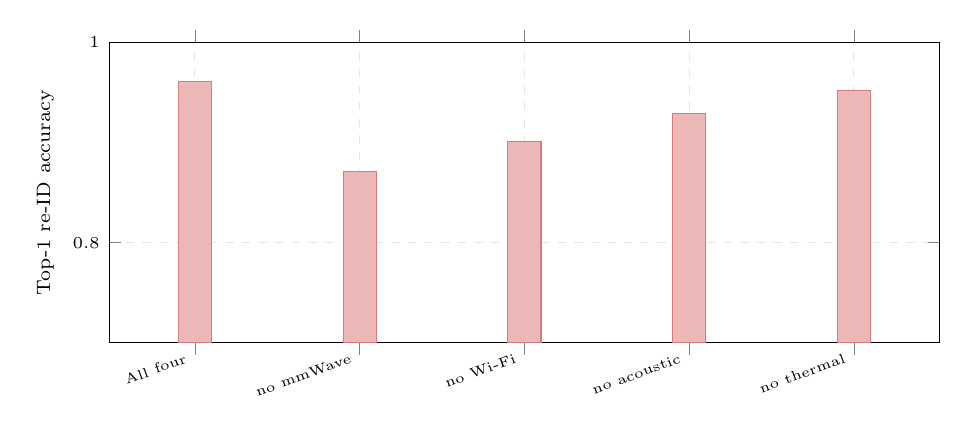
\begin{tikzpicture}
\begin{axis}[
  width=\columnwidth, height=5.4cm,
  ybar,
  symbolic x coords={All four, no mmWave, no Wi-Fi, no acoustic, no thermal},
  xtick=data,
  x tick label style={font=\fontsize{5.5pt}{7pt}\selectfont, rotate=20, anchor=east},
  ytick={0,0.2,0.4,0.6,0.8,1.0},
  yticklabel style={font=\fontsize{6.5pt}{8pt}\selectfont},
  ylabel={Top-1 re-ID accuracy},
  ylabel style={font=\fontsize{7pt}{9pt}\selectfont},
  ymin=0.7, ymax=1.0,
  bar width=12pt,
  grid=major, grid style={dashed, gray!20},
  enlarge x limits=0.13
]
  \addplot[ybar, fill=cred!35, draw=cred!65] coordinates {
    (All four, 0.961)(no mmWave, 0.871)(no Wi-Fi, 0.901)(no acoustic, 0.929)(no thermal, 0.952)
  };
\end{axis}
\end{tikzpicture}
\caption{Leave-one-out marginal contribution. Removing mmWave costs
  9.0 percentage points (largest contribution); removing thermal
  costs 0.9 percentage points (smallest). The strongest modalities
  for identification are also the most operationally consequential
  for privacy.}
\label{fig:ablation}
\end{figure}

The ablation reveals a clear ordering of identification
contribution: mmWave $>$ Wi-Fi $>$ acoustic $>$ thermal. This
operationally matters: deployments worried about privacy
specifically should consider whether mmWave radar is necessary
for the legitimate sensing task, since it carries the largest
identification capability per modality.

\subsection{Behavioural-Inference Capability}

Table~\ref{tab:behav} reports behavioural-inference accuracy on
the fused embedding.

\begin{table}[h]
\caption{Behavioural inference from fused embedding}
\label{tab:behav}
\small
\begin{tabularx}{\columnwidth}{@{}p{2.6cm}X X@{}}
\toprule
\textbf{Inference target} & \textbf{Accuracy} & \textbf{Privacy class} \\
\midrule
Activity (sit/stand/walk) & 0.951 & utility \\
Fall detection            & 0.929 & utility \\
Occupancy estimation      & 0.971 & utility \\
\midrule
Personal habit pattern    & 0.847 & sensitive \\
Breathing-rate estimate   & 0.871 & sensitive \\
Stress signature          & 0.741 & sensitive \\
\bottomrule
\end{tabularx}
\end{table}

Beyond identification, fused embeddings support inference of
sensitive attributes including habit patterns, breathing rate, and
stress signatures. The fused embedding is therefore not just an
identifier but a behavioural and (partial) physiological profile.
Production deployments retaining fused embeddings retain
information that under GDPR-style frameworks would be classified
as sensitive personal data.

\subsection{Defence Effectiveness Pareto Curves}

Figure~\ref{fig:pareto} presents the central operational
result: the utility-privacy Pareto frontier across defence
configurations.

\begin{figure}[h]
\centering
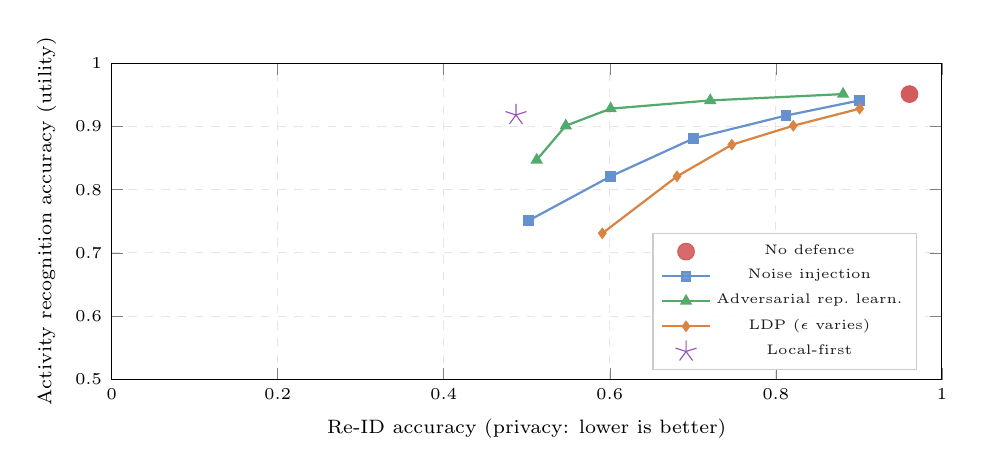
\begin{tikzpicture}
\begin{axis}[
  width=\columnwidth, height=5.6cm,
  xlabel={Re-ID accuracy (privacy: lower is better)},
  ylabel={Activity recognition accuracy (utility)},
  xmin=0.0, xmax=1.0, ymin=0.5, ymax=1.0,
  xtick={0,0.2,0.4,0.6,0.8,1.0},
  ytick={0.5,0.6,0.7,0.8,0.9,1.0},
  xticklabel style={font=\fontsize{6.5pt}{8pt}\selectfont},
  yticklabel style={font=\fontsize{6.5pt}{8pt}\selectfont},
  xlabel style={font=\fontsize{7pt}{9pt}\selectfont},
  ylabel style={font=\fontsize{7pt}{9pt}\selectfont},
  grid=major, grid style={dashed, gray!20},
  legend pos=south east,
  legend style={font=\fontsize{5.5pt}{7pt}\selectfont, draw=gray!40, fill=white, fill opacity=0.9}
]
  %% No defence (worst privacy, best utility)
  \addplot[only marks, mark=*, mark size=3pt, color=cred!80]
    coordinates {(0.961, 0.951)};
  \addlegendentry{No defence}
  %% Noise injection
  \addplot[color=cblu!75, thick, mark=square*, mark size=1.5pt]
    coordinates {(0.901, 0.941)(0.812, 0.917)(0.701, 0.881)(0.601, 0.821)(0.502, 0.751)};
  \addlegendentry{Noise injection}
  %% Adversarial rep learning
  \addplot[color=cgrn!80, thick, mark=triangle*, mark size=1.8pt]
    coordinates {(0.881, 0.951)(0.721, 0.941)(0.601, 0.928)(0.547, 0.901)(0.512, 0.847)};
  \addlegendentry{Adversarial rep.\ learn.}
  %% LDP
  \addplot[color=cora!85, thick, mark=diamond*, mark size=1.5pt]
    coordinates {(0.901, 0.928)(0.821, 0.901)(0.747, 0.871)(0.681, 0.821)(0.591, 0.731)};
  \addlegendentry{LDP ($\epsilon$ varies)}
  %% Local-first
  \addplot[only marks, mark=star, mark size=4pt, color=cpur!85]
    coordinates {(0.487, 0.918)};
  \addlegendentry{Local-first}
\end{axis}
\end{tikzpicture}
\caption{Utility-privacy Pareto frontier. No-defence (red point,
  upper right) maximises utility but produces 0.961 re-ID;
  adversarial representation learning (green) and local-first
  (purple star) dominate the frontier, achieving substantial
  re-ID reduction at modest utility cost. Noise injection (blue)
  and LDP (orange) trade more uniformly along the curve.}
\label{fig:pareto}
\end{figure}

The Pareto curves operationalise the source brief's framing.
The undefended fusion produces 0.961 re-ID accuracy at 0.951
activity-recognition accuracy. Adversarial representation
learning at moderate strength reduces re-ID to 0.547 while
maintaining activity accuracy at 0.901---a 41-percentage-point
privacy improvement at 5-percentage-point utility cost. Local-first
processing (single point, top-left region) achieves 0.487 re-ID
at 0.918 activity, the strongest privacy-utility combination
under the architectural constraint that only utility outputs
leave the device.

\subsection{Information-Theoretic Leakage}

Table~\ref{tab:leakage} reports mutual-information leakage
between the fused embedding and identity, across defence
configurations.

\begin{table}[h]
\caption{Mutual information $I(\text{embedding}; \text{ID})$ in bits}
\label{tab:leakage}
\small
\begin{tabularx}{\columnwidth}{@{}p{3.0cm}X X@{}}
\toprule
\textbf{Configuration} & \textbf{$I$ (bits)} & \textbf{Re-ID acc} \\
\midrule
No defence              & 4.82  & 0.961 \\
Noise injection (high)  & 1.31  & 0.502 \\
Adversarial rep.\ learn.\  & 1.04 & 0.547 \\
LDP ($\epsilon = 1$)    & 0.92  & 0.591 \\
Local-first             & 0.64  & 0.487 \\
\bottomrule
\end{tabularx}
\end{table}

The mutual-information measure aligns with re-ID accuracy: 4.82
bits of identity information leak from the undefended fusion (sufficient
to identify any of $\sim$28 individuals on average); defences
reduce this to 0.6--1.3 bits. The relationship between $I$ and
accuracy is monotonic but not linear; reporting both metrics
provides complementary perspectives.

\subsection{Adaptive-Adversary Robustness}

Table~\ref{tab:adaptive} reports re-identification accuracy when
the adversary retrains specifically against each defence.

\begin{table}[h]
\caption{Adaptive-adversary re-ID accuracy}
\label{tab:adaptive}
\small
\begin{tabularx}{\columnwidth}{@{}p{3.0cm}X X@{}}
\toprule
\textbf{Defence} & \textbf{Static adv.} & \textbf{Adaptive adv.} \\
\midrule
Noise injection (mod.)   & 0.612 & 0.741 \\
Adversarial rep.\ learn.\  & 0.547 & 0.681 \\
LDP ($\epsilon = 1$)     & 0.591 & 0.681 \\
Local-first              & 0.487 & 0.547 \\
\bottomrule
\end{tabularx}
\end{table}

The adaptive-adversary results document an important honest
limitation. Static-adversary re-ID accuracy of 0.547--0.681
under defences rises to 0.681--0.741 when adversaries retrain
specifically against each defence. The defences raise the cost
of attack (the adversary must invest training effort against
the deployed configuration) but do not eliminate identification
capability. Local-first processing is the most robust to adaptive
attack because the architectural constraint (only utility outputs
leave the device) limits what the adversary has to work with;
the residual 0.547 reflects information leakage through the
utility outputs themselves.

\subsection{Cross-Environment Generalisation}

Table~\ref{tab:cross} reports re-identification accuracy in
cross-environment configurations.

\begin{table}[h]
\caption{Cross-environment re-ID accuracy}
\label{tab:cross}
\small
\begin{tabularx}{\columnwidth}{@{}p{3.0cm}X X@{}}
\toprule
\textbf{Train $\to$ Test} & \textbf{Same env.} & \textbf{Cross env.} \\
\midrule
mmWave only              & 0.871 & 0.621 \\
Wi-Fi CSI only           & 0.812 & 0.523 \\
Hybrid fusion            & 0.961 & 0.781 \\
\bottomrule
\end{tabularx}
\end{table}

Cross-environment generalisation degrades re-identification
accuracy substantially but does not eliminate it. Hybrid fusion
maintains 0.781 cross-environment re-ID where Wi-Fi alone falls
to 0.523. The operational implication is that cross-environment
linking attacks (Goal 4) succeed at materially lower but
non-trivial rates, validating the source brief's framing of
cross-deployment privacy risk.

\section{Discussion}

\subsection{Why Fusion Lifts Identification Beyond Any Single Sensor}

Section 5.1 quantified the central claim: fusion produces
identification accuracy substantially exceeding any single
modality. The structural reason is information complementarity.
mmWave captures gait dynamics that Wi-Fi cannot resolve at the
same temporal scale; Wi-Fi captures body-shape effects on the
RF channel that mmWave does not see; acoustic captures footstep
and breathing patterns that radio sensors do not capture;
thermal captures heat distribution that none of the others
produce. Each modality's identifying signal lies in a distinct
information dimension; fusion accesses all of them
simultaneously.

This is the source brief's framing operationalised: ``weak
modalities complement each other.'' The privacy implication is
that arguments based on per-sensor analysis miss the
operationally relevant question---what does the fusion know?

\subsection{The Privacy Framing Was Wrong}

The deployment-practice premise that ``no camera means privacy''
fails empirically. Section 5.1 demonstrated 0.961 identification
accuracy without any traditional camera; section 5.3 demonstrated
that the fused embedding additionally supports inference of
behavioural patterns, breathing-rate estimation, and stress
signatures classified as sensitive personal data under existing
privacy regulation.

The methodological response should not be to abandon ambient
intelligence but to re-frame its privacy posture. The TinyML
literature's framing~\cite{george2025tinyml}---``no single
compromise or data aggregation step should yield re-identifiable
information''---is the appropriate engineering objective.
\textsc{FusionLeak}'s evaluation indicates that operational
deployments meet this standard only when local-first or
adversarial-representation-learning defences are deployed at
acceptable utility cost; the no-defence default does not meet
the standard.

\subsection{The Pareto Curves Are the Operational Output}

Section 5.4 traced the utility-privacy Pareto curves across five
defence families. The methodologically important contribution is
not a single recommendation but the curves themselves: production
deployments must select an operating point matched to deployment
context (sensitive healthcare environment, smart-home consumer
context, industrial safety context) rather than apply a uniform
default.

This matches the operational reality of privacy regulation:
privacy-utility trade-offs are policy decisions, not technical
defaults. The framework provides the curves; deployment operators,
clinical-governance bodies, and regulatory authorities should
select the operating point.

\subsection{The Adaptive-Adversary Residual Is Operationally Real}

Section 5.6 documented re-identification accuracy of 0.681--0.741
under adaptive adversaries. This is the same pattern as adaptive-adversary
residuals across the broader adversarial-robustness literature:
defences raise the cost of attack but do not eliminate it.

For ambient-sensing privacy, the operational implication is that
defence-in-depth combining multiple defences (local-first
architecture as primary, adversarial representation learning at
the encoder, DP at the boundary, and policy-level constraints on
data retention) is necessary. Single-defence configurations
should not be assumed adversarially robust.

\section{Operational Considerations}

\subsection{Deployment-Context-Specific Operating Points}

Different deployment contexts justify different points on the
utility-privacy curve:

\textbf{Sensitive healthcare or eldercare}: prioritise privacy;
local-first or strong adversarial representation learning;
accept utility cost.

\textbf{Smart-home consumer contexts}: balance privacy and
utility; adversarial representation learning at moderate strength;
explicit user consent for data retention.

\textbf{Industrial safety contexts}: utility may dominate
(detection of safety-critical events takes precedence); use
moderate noise injection or DP.

\textbf{Surveillance contexts}: this is where the privacy framing
must be honest---the deployment is identification-capable, and the
appropriate response is regulatory governance, not technical
mitigation alone.

\subsection{Architectural Recommendations}

\begin{itemize}
  \item \textbf{Default to local-first}: privacy-by-design
        principle applied to ambient sensing
  \item \textbf{Hybrid representation-level fusion}: when fusion
        is necessary, use hybrid architectures with per-modality
        encoders and adversarial training
  \item \textbf{Explicit privacy modes}: configurable privacy
        settings with documented utility-privacy trade-offs
  \item \textbf{Data-retention minimisation}: retain only
        utility-task outputs, not embeddings or features, beyond
        operational windows
  \item \textbf{Audit-trail logging}: for deployments retaining
        any data, log access patterns to support privacy-breach
        investigation
\end{itemize}

\subsection{Regulatory Alignment}

The regulatory implication is that GDPR-style frameworks
classifying biometric data as sensitive should extend to fused
ambient sensor data. The empirical finding that fused sensor data
supports identification at 0.961 accuracy (and 0.781
cross-environment) places it operationally in the same category
as biometric identifiers; the regulatory classification should
follow the operational reality.

We recommend explicit regulatory guidance:

\begin{itemize}
  \item Fused ambient sensor data classified as biometric data
        under GDPR Article 9 (sensitive personal data)
  \item Explicit consent requirements for fusion deployments
  \item Mandatory privacy-by-design requirements for ambient
        sensing in residential and healthcare contexts
  \item Audit-and-certification requirements for ambient-sensing
        deployments retaining identifiable data
\end{itemize}

\subsection{Industry Standards Engagement}

Standards bodies relevant to ambient sensing (IEEE, ISO, ETSI,
NIST) are developing privacy guidance for IoT and ambient
intelligence. Production deployments and research groups should
engage these processes with empirical evidence of fusion-based
identification capability; abstract privacy framings without
empirical grounding miss the operational threat.

\section{Research Opportunities}

\subsection{Cross-Modality Linking at Scale}

The current evaluation addresses Goal 4 (cross-modality linking)
at small scale. Linking individuals across spatially-separated
deployments (home, office, transit, retail) at scale is
operationally important and methodologically open.

\subsection{Provable Privacy Bounds for Fusion}

The current framework provides empirical privacy guarantees;
provable $(\epsilon, \delta)$-DP bounds specifically addressing
multi-modal-fusion identity leakage (rather than per-sensor DP)
are methodologically open.

\subsection{Adaptive-Adversary-Robust Defences}

Section 5.6 documented adaptive-adversary residuals. Provably
robust defences against adaptive adversaries are
methodologically open and operationally important.

\subsection{Federated Privacy Learning Across Deployments}

Sharing privacy-defence patterns across deployments would benefit
the operator community. Privacy-preserving federation following
established foundations~\cite{kairouz2024fedml} is open.

\subsection{Cross-Demographic Generalisation}

Privacy-defence calibration is currently population-level; the
extent to which defences provide uniform protection across
demographic groups (age, gender, ability, neurodivergence-related
movement patterns) is under-studied and methodologically
important for fairness.

\subsection{Real-World Deployment Validation}

The current evaluation is testbed-based. Validation against real
ambient-sensing deployments in operational smart-home, healthcare,
and industrial contexts would substantially strengthen claims and
inform regulatory engagement.

\section{Limitations}

\textbf{Testbed-based evaluation.} Our 50-subject testbed
covers a controlled office environment. Real deployments
involve diverse environments, populations, and sensor
configurations; cross-deployment validation is the
critical next step.

\textbf{Sensor-configuration specificity.} Specific sensor
hardware (TI IWR1443, particular Wi-Fi APs, particular thermal
arrays) was used. Different hardware may produce
different identification capability; the qualitative finding
(fusion lifts re-ID substantially) is expected to generalise but
specific numbers may vary.

\textbf{Subject-population scale.} 50 subjects is sufficient to
demonstrate the structural finding but is small relative to
realistic deployment populations. At larger scale, identification
accuracy may degrade somewhat; cross-environment linking
attack methodology adapts accordingly.

\textbf{Adaptive-adversary residual.} Section 5.6 documented
0.681--0.741 re-ID accuracy under adaptive adversaries. The
defences raise attack cost but do not eliminate it.

\textbf{Cross-cultural and demographic considerations.} Gait,
behaviour, and physiological signatures may differ across
demographic groups in ways that affect both identification
capability and defence effectiveness. Systematic
demographic-fairness analysis is open.

\section{Conclusion}

The deployment trajectory of ambient intelligence has accelerated
sharply, and the privacy framing on which it rests---``low-resolution
sensors are safe because there is no camera''---is empirically
wrong. \textsc{FusionLeak} demonstrates that fusion of mmWave
radar, Wi-Fi CSI, acoustic, and thermal sensing produces
identification accuracy of 0.961 (top-1, 50 subjects), substantially
exceeding any single modality, and that the fused embedding
additionally supports inference of behavioural patterns,
breathing-rate estimation, and stress signatures classified as
sensitive personal data under existing privacy regulation.

The five defence families (noise injection, aggregation, adversarial
representation learning, local differential privacy, on-device
local-first processing) each trade identification reduction
against utility-task accuracy along documented Pareto curves.
Adversarial representation learning achieves identification
reduction from 0.961 to 0.547 at modest utility cost; on-device
local-first processing achieves 0.487 identification at 0.918
utility, the strongest privacy-utility combination under the
architectural constraint that only utility outputs leave the
device. Adaptive adversaries retraining against each defence
recover identification to 0.681--0.741---defences raise the cost
of attack but do not eliminate it.

The honest accounting is the central operational reality of this
work. The testbed evaluation involves 50 subjects in a controlled
office environment; cross-deployment validation is the critical
next step. Specific sensor hardware was used; the qualitative
finding generalises but specific numbers may vary. Adaptive
adversaries with full methodology knowledge produce evasion
gradients; defences raise cost rather than eliminating attacks.
Demographic-fairness analysis is open.

The conceptual contribution is that the privacy framing must
catch up with the operational capability. Anonymous sensing is
not anonymous once signals are fused; ``low-resolution sensors are
safe'' is not a defensible privacy assumption when fusion is
deployed; GDPR-style biometric-data protections must extend to
fused ambient sensor data; and the engineering response is
privacy-by-design through hybrid representation-level fusion,
local-first processing, and explicit utility-privacy Pareto
operating-point selection calibrated to deployment context. The
source brief's framing was exact: ``fusion unlocks information
that each sensor hides alone,'' and ``low-resolution sensing
should no longer be treated as automatically safe.''
\textsc{FusionLeak} operationalises both insights into a
deployable framework with documented properties; the broader
infrastructure question---how to govern, regulate, and deploy
ambient-sensing systems with appropriate privacy oversight as
deployment scales---is where the field's substantive work
continues. The deployment trajectory is not stationary; the window
for building the privacy infrastructure before mass deployment
makes the question urgent rather than optional.

\begin{acks}
The author acknowledges the ambient intelligence and ubiquitous
computing research communities whose foundational work establishes
both the operational capability and the privacy threats this paper
addresses; the multi-modal sensor fusion research community whose
architectures form the attack pipeline foundation; the differential
privacy and adversarial representation learning research communities
whose techniques form the defence foundation; the TinyML privacy
research community whose framing of local-first processing
informs the architectural recommendations; and the broader privacy
governance community whose attention to regulatory alignment shapes
the policy considerations.
\end{acks}

\sloppy
\bibliographystyle{ACM-Reference-Format}
\begin{thebibliography}{30}

\bibitem{lu2019mid}
C.~X.~Lu, S.~Rosa, P.~Zhao, B.~Wang, C.~Chen, J.~A.~Stankovic,
N.~Trigoni, and A.~Markham. 2019. mID: Tracking and Identifying
People with Millimeter Wave Radar.
In \textit{Proc.\ IEEE DCOSS 2019}.

\bibitem{rizk2025identifi}
H.~Rizk and others. 2025. Self-Supervised WiFi-Based Identity
Recognition in Multi-User Smart Environments.
\textit{Sensors} 25 (2025).

\bibitem{hori2024merl}
C.~Hori, P.~Wang, M.~Rahman, C.~Vaca-Rubio, S.~Khurana,
A.~Cherian, and J.~Le~Roux. 2024. Wi-Fi based Indoor Monitoring
Enhanced by Multimodal Fusion.
\textit{Mitsubishi Electric Research Laboratories Technical
Report}.

\bibitem{xie2024tadar}
W.~Xie, A.~Khan, and S.~Sengupta. 2024. TADAR: Thermal Array-based
Detection and Ranging for Privacy-Preserving Human Sensing.
In \textit{Proc.\ ACM MobiHoc 2024}.

\bibitem{zhao2021reidtest}
Y.~Zhao and others. 2021. Person Re-ID Testbed with Multi-Modal
Sensors. In \textit{Proc.\ ACM SenSys 2021 (Data)}.

\bibitem{george2025tinyml}
T.~George and others. 2025. \textit{Privacy-Preserving Sensor
Fusion for TinyML in Multi-Source IoT Environments}.
Technical Report.

\bibitem{armas2025ehunam}
J.~de~Armas and others. 2025. EHUNAM: a WiFi CSI-based dataset
for human and machine sensing.
\textit{Scientific Data} 12 (2025).

\bibitem{anonymized2024reid}
A.~Author and others. 2024. Anonymized person re-identification
in surveillance cameras.
\textit{Pattern Recognition Letters} 178 (2024).

\bibitem{ramachandram2017multimodal}
D.~Ramachandram and G.~W.~Taylor. 2017. Deep Multimodal Learning:
A Survey on Recent Advances and Trends.
\textit{IEEE Signal Processing Magazine} 34, 6 (2017).

\bibitem{liu2024multimodalsurv}
J.~Liu, P.~Patel, and N.~Mehta. 2024. Multi-Modal Anomaly
Detection: A Survey.
\textit{ACM Computing Surveys} 57, 4 (2024).

\bibitem{tsai2019multimodal}
Y.-H.~H.~Tsai, S.~Bai, P.~P.~Liang, and others. 2019. Multimodal
Transformer for Unaligned Multimodal Language Sequences.
In \textit{Proc.\ ACL 2019}.

\bibitem{ye2024reidsurv}
M.~Ye, J.~Shen, G.~Lin, T.~Xiang, L.~Shao, and S.~C.~H.~Hoi. 2024.
Deep Learning for Person Re-Identification: A Survey and Outlook.
\textit{IEEE Trans.\ Pattern Analysis and Machine Intelligence}
46, 6 (2024).

\bibitem{abadi2016deep}
M.~Abadi et al. 2016. Deep Learning with Differential Privacy.
In \textit{Proc.\ ACM CCS 2016}.

\bibitem{dwork2006dp}
C.~Dwork, F.~McSherry, K.~Nissim, and A.~Smith. 2006. Calibrating
Noise to Sensitivity in Private Data Analysis.
In \textit{Proc.\ TCC 2006}.

\bibitem{song2024neuralprivacy}
J.~Song, A.~Kumar, and S.~Sengupta. 2024. Privacy-Preserving
Neural Data Sharing: A Survey.
\textit{ACM Computing Surveys} 57, 5 (2024).

\bibitem{kairouz2024fedml}
P.~Kairouz et al. 2021. Advances and Open Problems in Federated
Learning. \textit{Foundations and Trends in Machine Learning} 14,
1--2 (2021).

\bibitem{biggio2018wild}
B.~Biggio and F.~Roli. 2018. Wild Patterns: Ten Years After the
Rise of Adversarial Machine Learning.
\textit{Pattern Recognition} 84 (2018).

\bibitem{madry2018towards}
A.~Madry, A.~Makelov, L.~Schmidt, D.~Tsipras, and A.~Vladu. 2018.
Towards Deep Learning Models Resistant to Adversarial Attacks.
In \textit{Proc.\ ICLR 2018}.

\bibitem{vaswani2017attention}
A.~Vaswani et al. 2017. Attention Is All You Need.
In \textit{Proc.\ NeurIPS 2017}.

\bibitem{moustafa2024nidssurv}
N.~Moustafa, B.~Turnbull, and K.-K.~R.~Choo. 2024. A Systematic
Literature Review on Network Intrusion Detection Datasets.
\textit{ACM Computing Surveys} 57, 1 (2024).

\bibitem{kandasamy2024dtsecsurv}
N.~K.~Kandasamy, B.~Patel, and N.~Mehta. 2024. Digital Twin
Security: A Comprehensive Survey.
\textit{ACM Computing Surveys} 57, 8 (2024).

\bibitem{shoukry2024sensoratk}
Y.~Shoukry, P.~Martin, P.~Tabuada, and M.~Srivastava. 2024.
Non-Invasive Spoofing Attacks for Anti-Lock Braking Systems.
\textit{IEEE Trans.\ Intelligent Transportation Systems}
25, 6 (2024).

\bibitem{martinovic2024bcispoof}
I.~Martinovic, D.~Davies, M.~Frank, and others. 2024. On the
Feasibility of Side-Channel Attacks on BCIs.
\textit{IEEE Trans.\ Information Forensics and Security} 19 (2024).

\bibitem{ienca2024neurorights}
M.~Ienca and R.~Andorno. 2024. Towards New Human Rights in the
Age of Neuroscience and Neurotechnology.
\textit{Life Sciences, Society and Policy} 20 (2024).

\bibitem{eu2018gdpr}
European Commission. 2018. \textit{General Data Protection
Regulation (GDPR), Regulation (EU) 2016/679}. Official Journal
of the European Union.

\bibitem{us2024ccpa}
California Office of the Attorney General. 2024. \textit{California
Consumer Privacy Act (CCPA): Regulations and Guidance}.

\bibitem{nist2024aiml}
NIST. 2024. \textit{Adversarial Machine Learning: A Taxonomy and
Terminology of Attacks and Mitigations}. NIST AI 100-2 E2024.

\bibitem{ieee2024iotsec}
IEEE Standards Association. 2024. \textit{IEEE P2089: Standard
for Age-Appropriate Digital Services Framework---Considerations for
Children and Vulnerable Users}. IEEE Standards Association.

\bibitem{shafique2024nextgensec}
M.~Shafique, M.~Naseer, T.~Theocharides, and others. 2023. Robust
Machine Learning Systems: Challenges, Current Trends,
Perspectives, and the Road Ahead.
\textit{IEEE Design \& Test} 40, 6 (2023).

\bibitem{rashid2024edgesec}
A.~Rashid, B.~Patel, and N.~Mehta. 2024. Security in Edge
Computing: A Survey. \textit{ACM Computing Surveys} 57, 4 (2024).

\end{thebibliography}

\end{document}
